\subsection{Servidor}

Para levantar un servidor, se requiere que se ejecute la siguiente linea:

\lstset{
	language=Bash, 
    commentstyle=\color{commentgreen},
    keywordstyle=\color{eminence},
    stringstyle=\color{red},
    basicstyle=\small\ttfamily, % basic font setting
    emph={int,char,double,float,unsigned,void,bool,NULL},
    emphstyle={\color{blue}},
    escapechar=\&,
    breaklines=true,
    numbers=left,
    numberstyle=\tiny, 
    stepnumber=1, 
    numbersep=-2pt
    % keyword highlighting
    }
\begin{lstlisting}[frame=single, caption=Instalación de dependencias, label=code:openServer]
	worms_server <PORT>
\end{lstlisting}

Donde el puerto debe ser mayor a 1000 si es que no se quiere ejecutar el comando como \texttt{sudo}. Además, si se quiere realizar cambios en la configuración del juego, es necesario reiniciar le servidor, para que este vuelva a leer el archivo correspondiente y cargar los datos necesarios. 

El archivo \texttt{serverConfig.yaml}, que se encuentra en \texttt{/etc/Worms}, tiene la información para configurar la experiencia de juego. En este archivo se pueden modificar parámetros como los tiempos de los turnos (\emph{turnTime}, \emph{extraTurnTime}, \emph{waitForNextTurnTime}, \emph{teleportTime}), como también la distancia de caida que puede realizar el gusano sin recibir daño (\emph{safeFallDistance}), su daño maximo, etc. También se pueden modificar parámetros de las armas, como lo pueden ser el daño de esta, el radio del impacto, el factor de amortiguamiento de las explosiones (cuanto impulso se le asigna al gusano impactado), el tiempo inicial para que explote, la friccion y rebote de la bala ( efecto que se apreciará si es un arma que no explota al primer contacto), etc.

Finalmente, para realizar un cierre con su liberación ordenada de los recursos, le usuario solo debe tipear la tecla q en la consola que se haya ejecutado el servidor. En la figura \ref{im:cierreS} se puede ver como se cierra dicho ejecutable.

\begin{figure}[H]
	\centering
	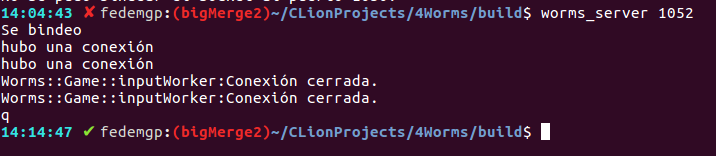
\includegraphics[scale=0.4]{cierreServer.png}
	\caption{Cierre ordenado del servidor}
	\label{im:cierreS}
\end{figure}


\subsection{Cliente}
En la figura \ref{im:juego} puede verse un cliente en pleno juego. En este pueden verse distintas cosas que merecen ser destacadas:

\begin{figure}[H]
	\centering
	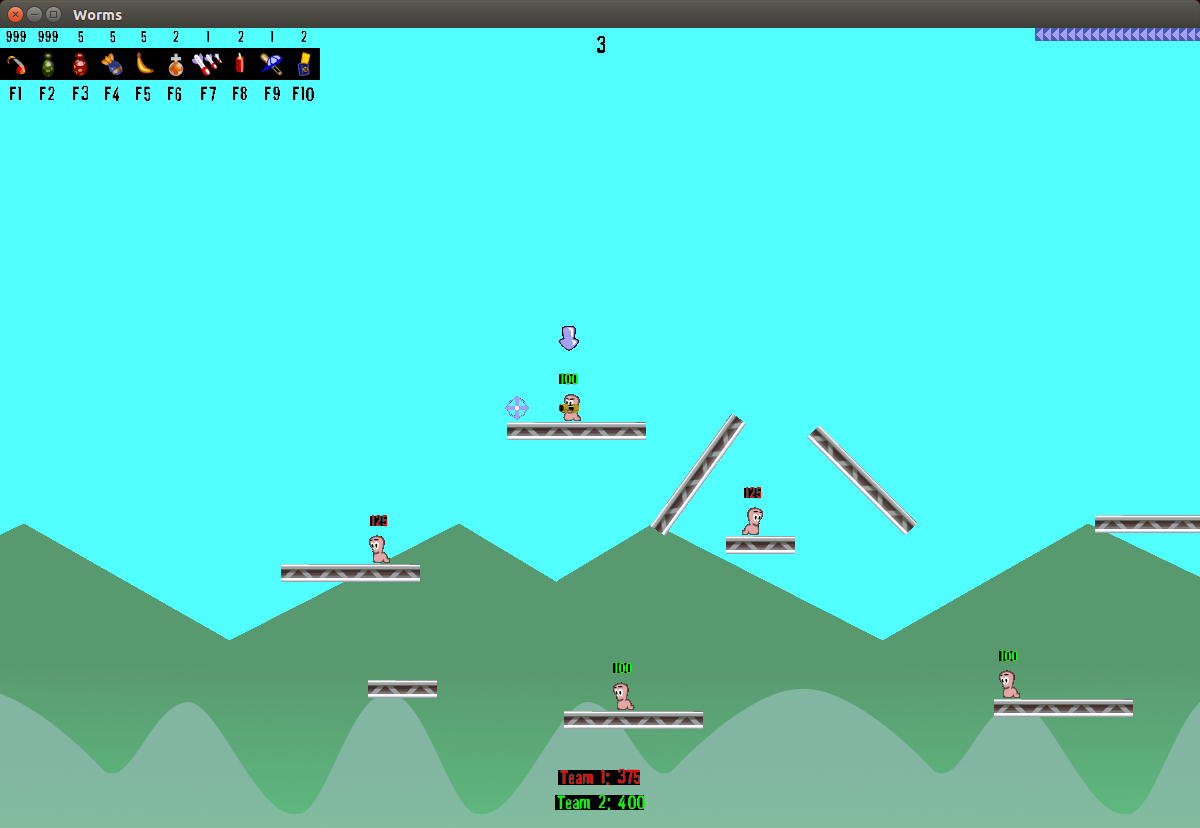
\includegraphics[scale=0.4]{game.png}
	\caption{Captura de una partida del Worms}
	\label{im:juego}
\end{figure}

\begin{itemize}
	\item En la esquina superior izquierda, puede verse el arsenal, en este se informa al usuario las armas disponibles, que botón se debe teclear para usar dicha arma (abajo del icono), y por encima del ícono, la cantidad de municiones que posee dicha arma. Cuando el contador llega a cero, el equipo no podrá usar mas esa arma.
	\item En la esquina superior derecha, puede verse una barra con flechas. Esa barra indica la intensidad del viento. Cuando mas larga la barra, mas fuerte será el viento. Además la flecha indica la dirección de este. Hay ciertas armas cuyas balas son afectadas por el viento. La intensidad de este y si la bala de un determinado arma es afectado por el viento puede editarse en el archivo mencionado previamente en la sección \ref{sec:config}. 
	\item Arriba al centro puede ver un contador. Este marca el tiempo de cada turno. Cuando un turno termina, se cuenta un periodo extra, donde se indica quien tiene el siguiente turno. El usuario, durante este período, no podrá moverse. Por default este período es de 3 segundos. Finalmente, cuando un gusano dispara, también se empieza a contar un tiempo determinado en donde se le permite al usuario moverse momentaneamente luego de disparar. Tanto el tiempo del turno, como el tiempo de espera al siguiente turno y el tiempo extra luego de disparar, puede configurarse en el archivo mencionado en la sección \ref{sec:config}.
	\item En la zona inferior de la ventana, se observa la vida total de cada equipo. Es la sumatoria de las vidas individuales de cada gusano. Cuando ese contador llega a cero, ese equipo pierde.
\end{itemize}

\subsubsection{Controles}
Para poder jugar al \emph{Worms}, el usuario puede usar las siguientes teclas:

\begin{itemize}
	\item \textbf{Espacio}: presionando dicha tecla, el worm comienza a cargar potencia para que la bala alcance una distancia mayor. Al soltar la barra, o al llegar al máximo de potencia, el disparo se realiza. Dicha tecla no tiene efecto en armas teledirigidas como la teleportación o el ataque aereo.
	\item \textbf{Enter}: realiza un salto hacia delante. La velocidad de este salto puede cambiarse en el archivo de configuración.
	\item \textbf{Retroceso}: realiza un salto mortal hacia atrás.
	\item \textbf{F1 - F10}: cambia el arma seleccionada de acuerdo al arsenal mencionado previamente.
	\item \textbf{1-5}: Cambia el tiempo de explosión de las distintas grandas (granada verde, cluster, holy, dinamita).\footnote{Vale la aclaración que no hay una notificación evidente cuando se cambia el tiempo de explosión. Por cuestiones de tiempo y prioridades se dejó ese feature para mas adelante. Sin embargo el timeout funciona.}
	\item \textbf{Flechas}: permiten mover al worm de izquierda a derecha, y con las flechas arriba y abajo se puede cambiar el ángulo de disparo de las distintas armas (si estas lo permiten).
	\item \textbf{Click izquierdo}: util para armas teledirgidas. Selecciona el punto a donde deben ir dichas herramientas / armas.
\end{itemize}

\subsubsection{Empezar una partida}
Para comenzar una partida, primero es necesario abrir un cliente. Esto se logra ejecutando desde consola el comando \texttt{worms\_client}. Luego, se debe conectar al servidor, para esto hay que ingresar el HOST y el PORT en la pantalla que se muestra en la figura \ref{im:conec}. 

\begin{figure}[H]
	\centering
	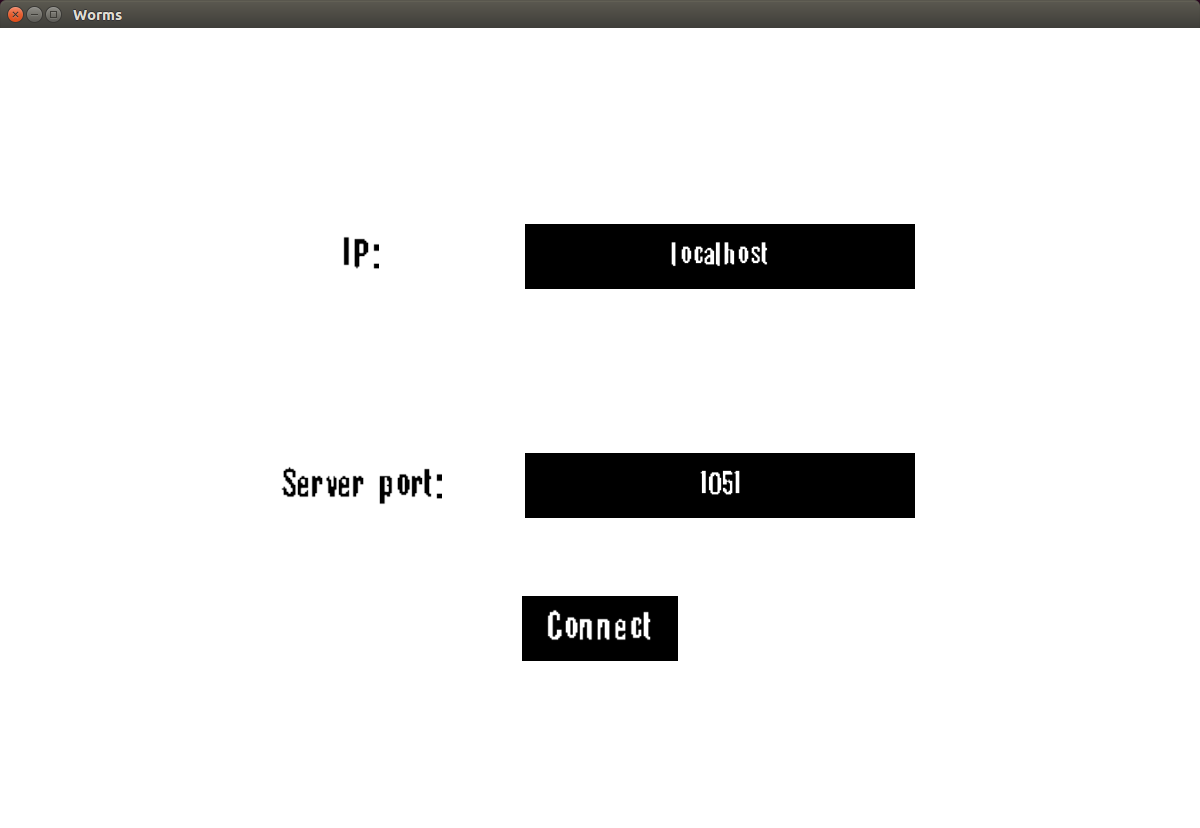
\includegraphics[scale=0.4]{clientConnection.png}
	\caption{Pantalla de conexión al servidor}
	\label{im:conec}
\end{figure}

Una vez conectado al servidor, este te da la opción de crear una partida nueva (figura \ref{im:create}), o de unirse a alguna ya existente (figura \ref{im:join}). Para la creación, se puede observar que cada nivel tiene prefijado la cantidad de jugadores que pueden conectarse a dicho nivel. 
 Por otro lado, para unirse a una partida, solo se podrá hacerlo en aquellas que no estén completas. 
 
\begin{figure}[H]
	\centering
	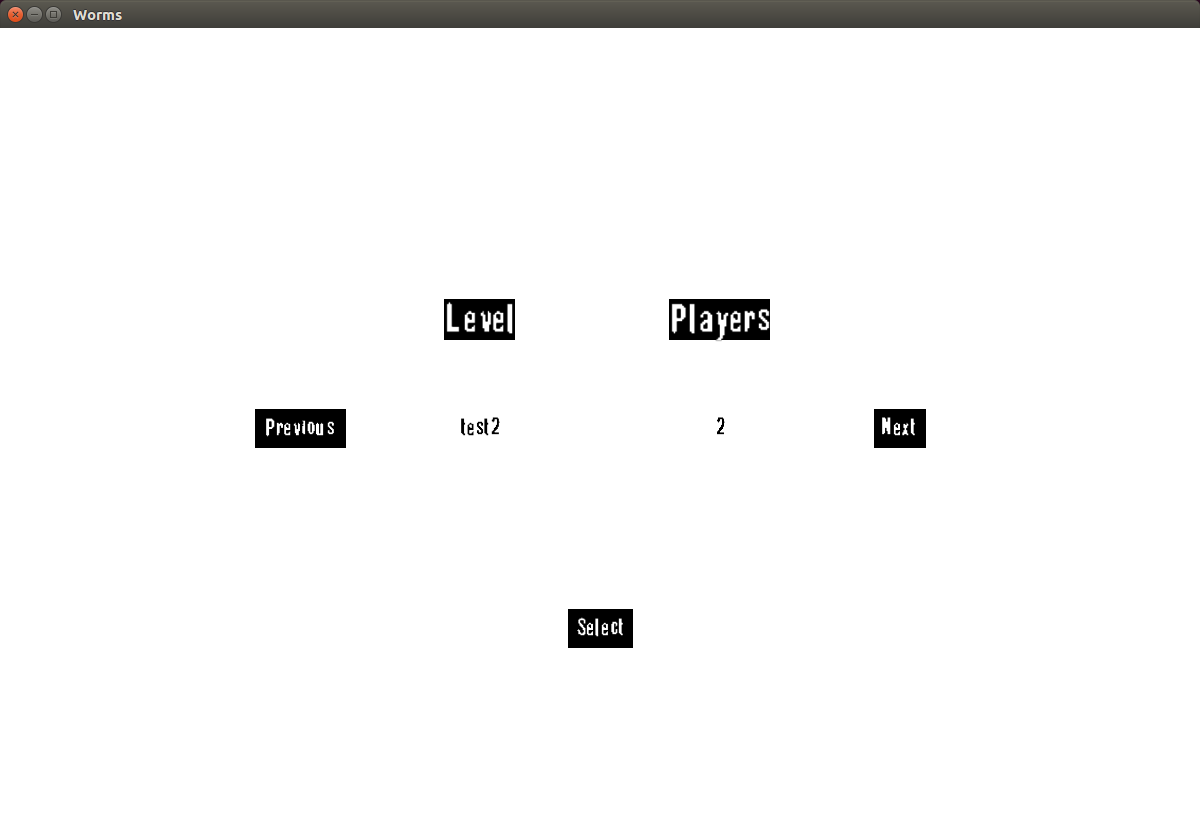
\includegraphics[scale=0.4]{createGames.png}
	\caption{Pantalla de elección de nivel para crear una partida.}
	\label{im:create}
\end{figure}

\begin{figure}[H]
	\centering
	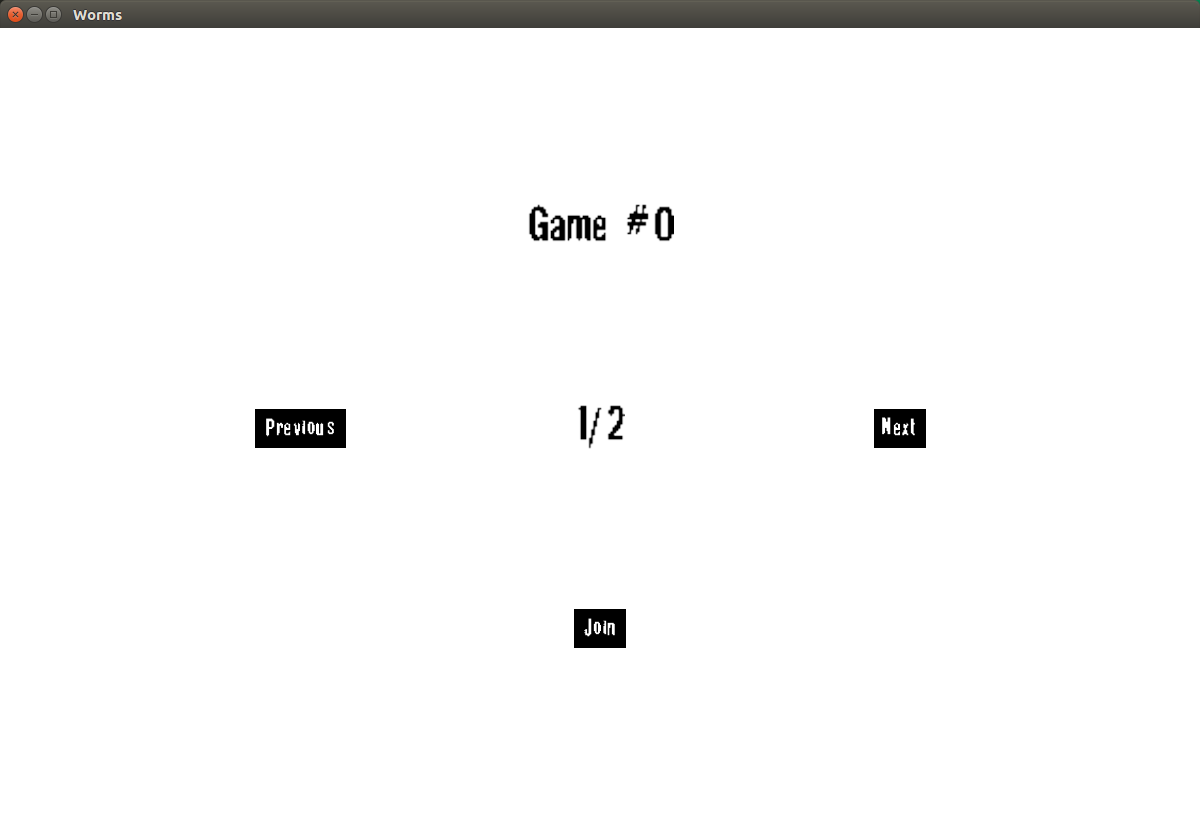
\includegraphics[scale=0.4]{joinGame.png}
	\caption{Pantalla de elección de sala para unirse a una partida.}
	\label{im:join}
\end{figure}

Una vez finalizada la partida, aparecerá una imagen de victoria/derrota dependiendo de tu desempeño (figura \ref{im:fin}).

\begin{figure}[H]
	\centering
	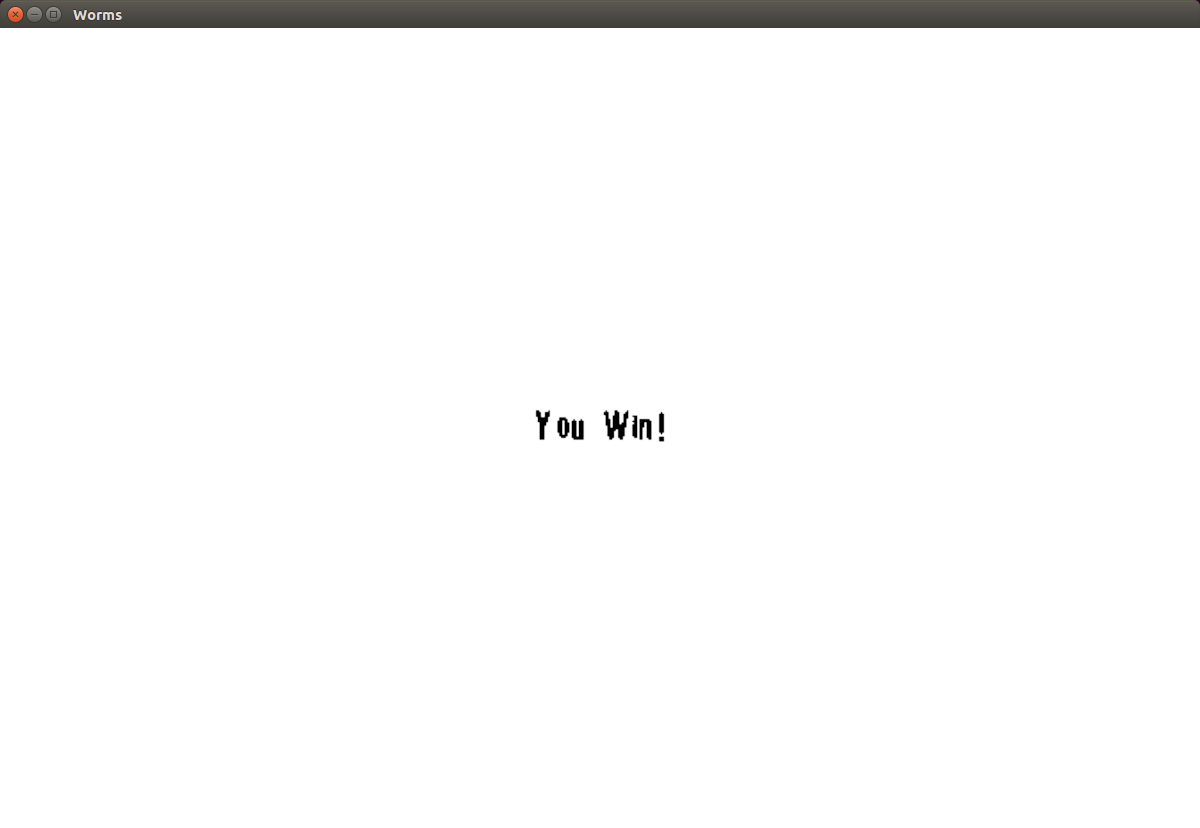
\includegraphics[scale=0.4]{endGame.png}
	\caption{Pantalla de victoria.}
	\label{im:fin}
\end{figure}

\subsection{Editor}
El editor puede abrirse ejecutando desde una consola el comando \texttt{worms\_editor}. En este se puede crear mapas, con dos tipos de vigas, a las cuales se las puede rotar, y se pueden colocar una cantidad determinada de gusanos. Además se pueden ajustar parámetros del juego como la vida de los worms, la cantidad de jugadores que permite este mapa, la duración del turno, y las municiones de cada arma. A continuación se listarán los distintos controles que tiene el editor:

\begin{itemize}
	\item \textbf{Click izquierdo}: Coloca una viga o un gusano en la zona seleccionada.
	\item \textbf{Click derecho}: Remueve una viga o un gusano.
	\item \textbf{Teclas + y -}: rotan las vigas.
	\item \textbf{W}: shortcut para posicionar gusanos.
	\item \textbf{L}: shortcut para posicionar vigas largas.
	\item \textbf{S}: shortcut para posicionar vigas cortas.
\end{itemize}

En la barra de herramientas, en la zona superior izquierda, se puede seleccionar backgrounds para el juego (hasta 3). Hay algunos predefinidos en \texttt{/var/Worms/assets/img/background}. Finalmente, se puede exportar el mapa en formato YAML en la sección \texttt{File -> export}. Para poder utilizar dicho mapa, debe copiarse el archivo creado en la dirección \texttt{/var/Worms/res/<folder>/}, donde <folder> es una carpeta con nombre a elección. Es necesario también reiniciar el servidor para que cargue dicho mapa. En la figura \ref{im:editor} puede verse una imagen de un mapa creado.

\begin{figure}[H]
	\centering
	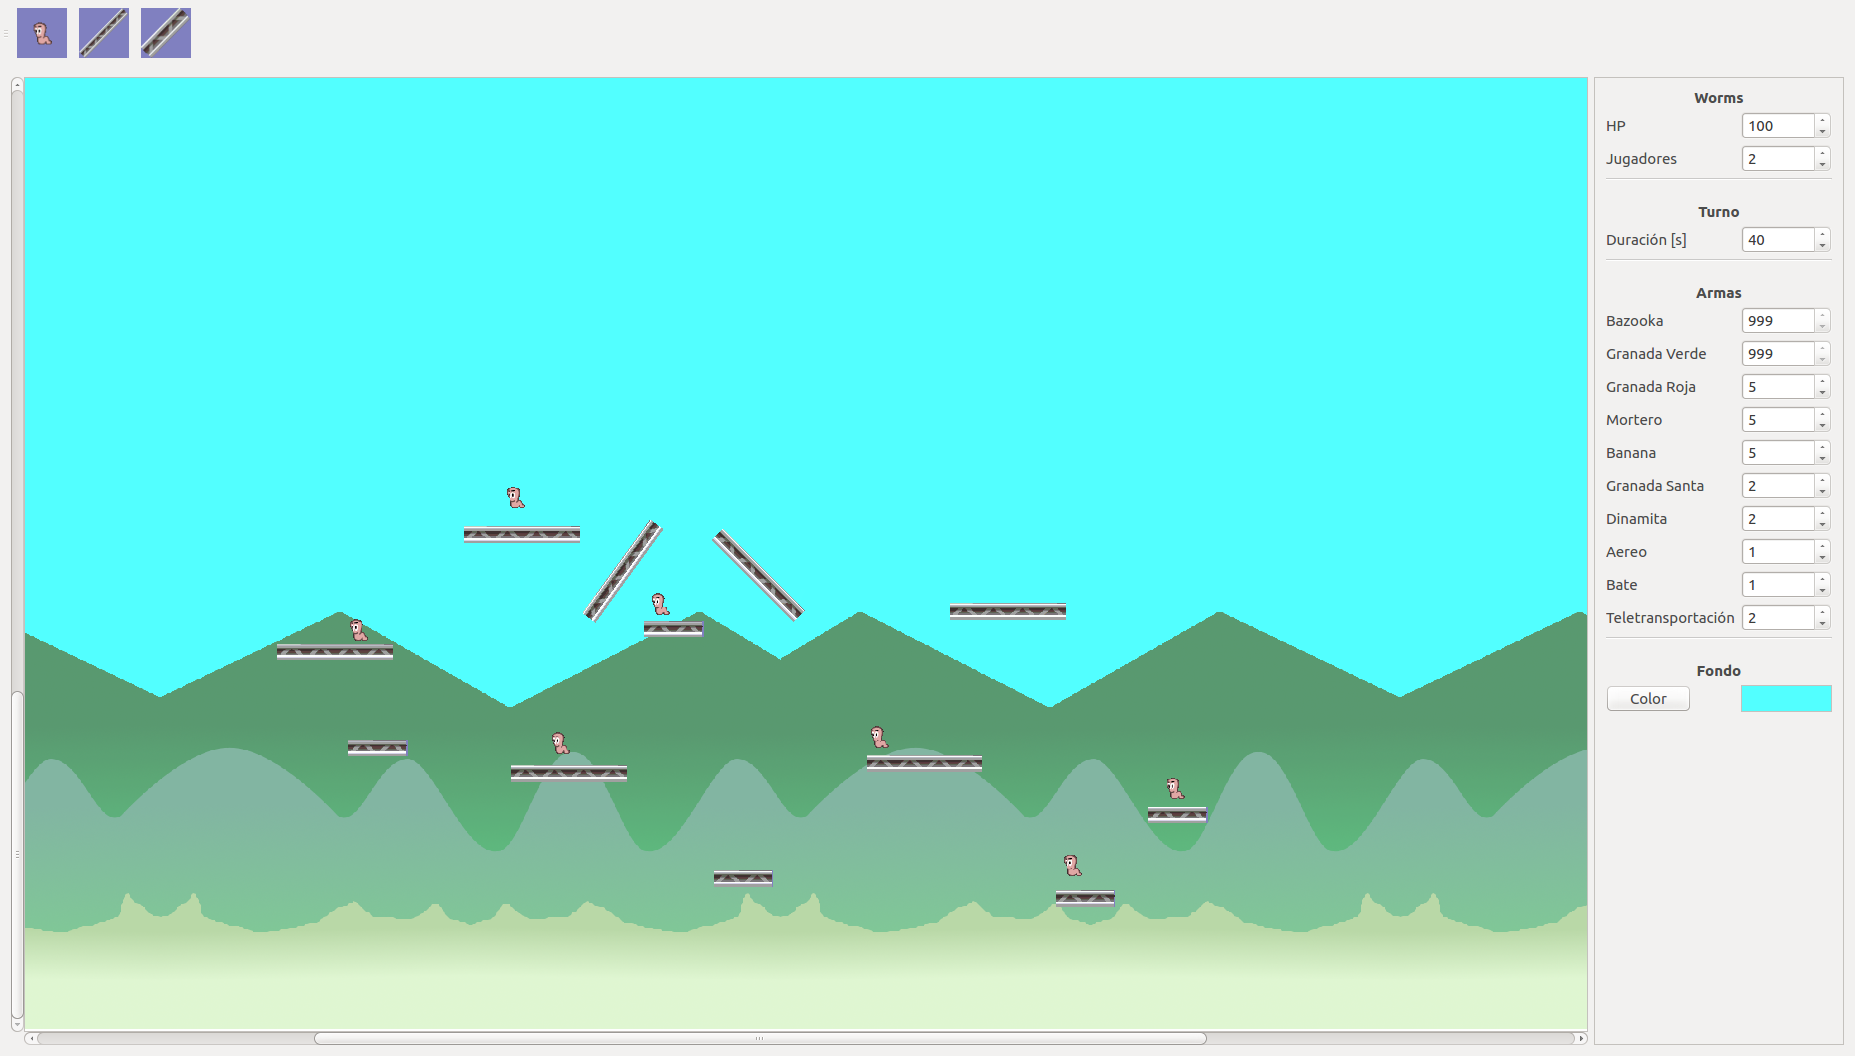
\includegraphics[scale=0.25]{editor1.png}
	\caption{Vista de un mapa terminado.}
	\label{im:editor}
\end{figure}